\documentclass{classrep}
\usepackage[utf8x]{inputenc}
\usepackage[a4paper, left=1.0cm, right=1.0cm, top=1.0cm, bottom=2.0cm, headsep=0.5cm, headheight=15pt]{geometry}
\usepackage{amsmath, amsthm, amssymb, amsfonts}
\usepackage{graphicx}
\usepackage{float}
\usepackage{hyperref}
\hypersetup{pdfborder={0 0 0 0}}

\studycycle{Elektronika i Telekomunikacja, studia dzienne, mgr II st.}
\coursesemester{II}
\coursename{Procesy stochastyczne w elektronice}
\courseyear{2015/2016}
\courseteacher{dr inż. Robert Hanus}
\coursegroup{środa, 12:00}

\author{  \studentinfo{Witold Olechowski}{127517} 	\and
		  \studentinfo{Grzegorz Pelczar}{125242} 	\and
		  \studentinfo{Tomasz Marecik}{127374} 		}

\title{\textbf{Zadanie:} Pomiar Opóźnienia Przy Zastosowaniu Charakterystyki Fazowej Wzajemnej Gęstości Widmowej Mocy }

%\lstinputlisting{block1.vhdl}
%\vskip 2\baselineskip

\begin{document}
\maketitle

\section{Cel ćwiczenia}
\quad Celem ćwiczenia jest poznanie zasady pomiaru małych opóźnień sygnałów losowych przy zastosowaniu charakterystyki fazowej wzajemnej gęstości widmowej mocy. Do przeprowadzenia niniejszego ćwiczenia należy wykorzystać oprogramowanie pakietu DASYLab. 

\section{Wyznaczanie wzajemnej gęstości widmowej mocy (WGWM)}
\quad Zbudowany został w programie DASYLab 9 układ przedstawiony na rys. \ref{fig:sch1}

\begin{figure}[H]
\centering
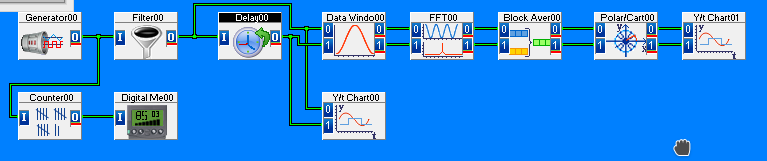
\includegraphics[width=0.8\linewidth]{sch1}
\caption{Układ do pomiaru gęstości widmowej mocy}
\label{fig:sch1}
\end{figure}

Funkcje modułów oraz menu programu zostały nastawione zgodnie z instrukcją. 

\subsection{Zaobserwowane zostały przebiegi modułu i fazy WGWM i ich zmiany w miarę wzrostu liczby uśrednień. Nastawy modułu Delay00 dla opóźnienia równego 2 ms pokazano na rys. \ref{fig:wyk1}, \ref{fig:wyk2}, \ref{fig:wyk3}  }

\begin{figure}[H]
\centering
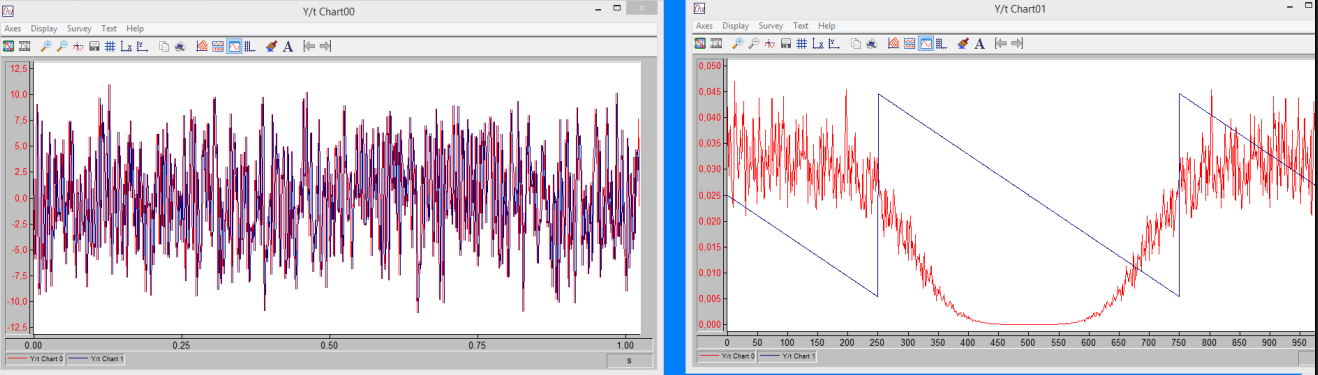
\includegraphics[width=1\linewidth]{wyk1}
\caption{Przebieg modułu i fazy WGWM przy opóźnieniu 2 ms dla liczba uśrednień równej 34.}
\label{fig:wyk1}
\end{figure}

\begin{figure}[H]
	\centering
	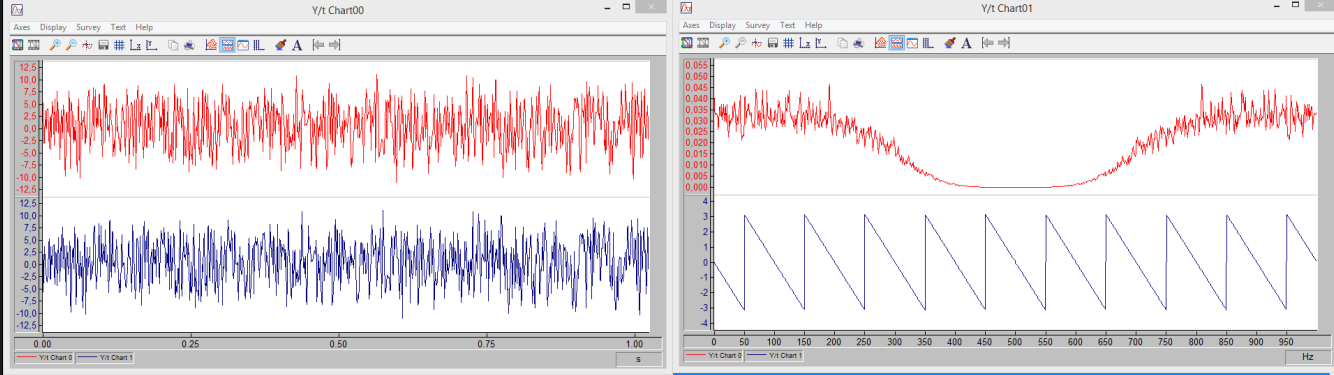
\includegraphics[width=1\linewidth]{wyk2}
	\caption{Przebieg modułu i fazy WGWM przy opóźnieniu 2 ms dla liczba uśrednień równej 50.}
	\label{fig:wyk2}
\end{figure}

\begin{figure}[H]
	\centering
	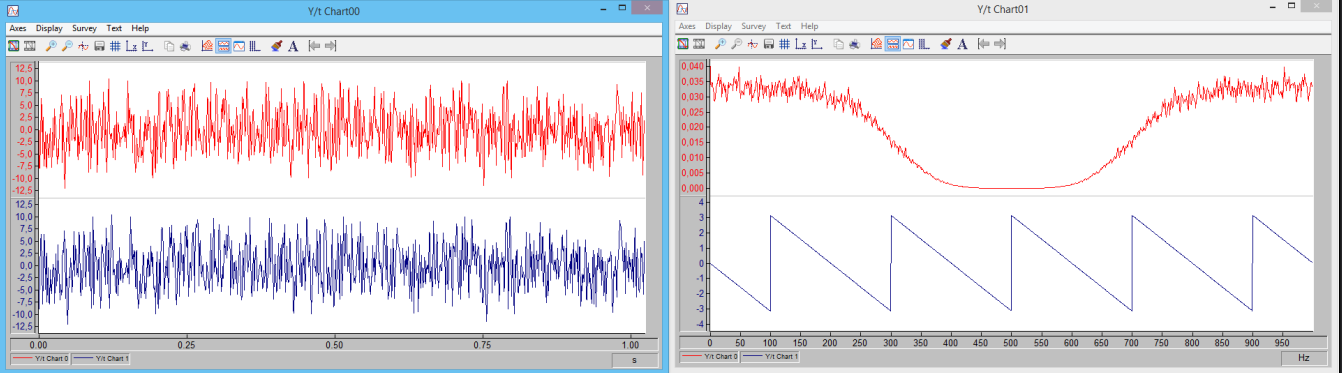
\includegraphics[width=1\linewidth]{wyk3}
	\caption{Przebieg modułu i fazy WGWM przy opóźnieniu 2 ms dla liczba uśrednień równej 217.}
	\label{fig:wyk3}
\end{figure}
\quad Przedstawione przebiegi modułu i fazy pokazały, że im wyższa liczba uśrednień tym bardziej zostały wygładzone wyznaczone charakterystyki.


\section{Zastosowanie charakterystyki fazowej wzajemnej gęstości widmowej mocy do
	pomiaru opóźnienia}

\quad Układ z rys. \ref{fig:sch1}  rozbudowano o dodatkowe moduły (rys. \ref{fig:sch2})

\begin{figure}[H]
	\centering
	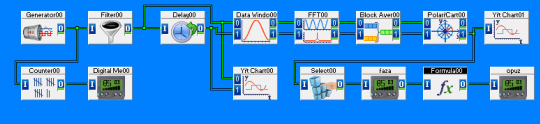
\includegraphics[width=0.8\linewidth]{sch2}
	\caption{Układ do wyznaczania opóźnienia na podstawie charakterystyki fazowej WGWM.}
	\label{fig:sch2}
\end{figure}

Funkcje modułów oraz menu programu zostały nastawione zgodnie z instrukcją.  

\subsection{Dla nastaw modułów Delay00:  Delay Data by 0,002 Seconds, Slider00: 200 uruchomiono program i zaobserwowano wskazania mierników.}

\begin{figure}[H]
\centering
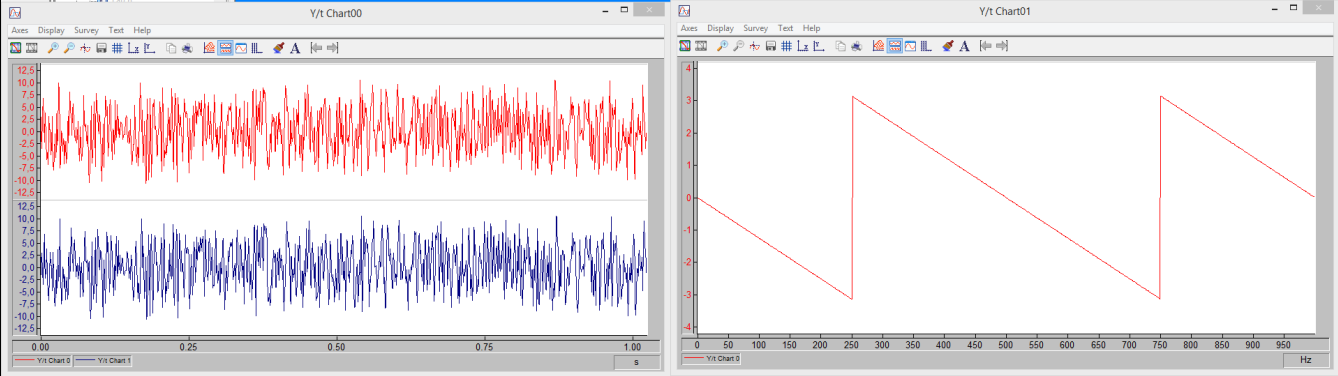
\includegraphics[width=1\linewidth]{wyk4}
\caption{Charakterystyka fazowa WGWM, dla częstotliwości 200Hz. Opóźnienie równe $1,9972ms$, faza równa $-2,57rad$}
\label{fig:wyk4}
\end{figure}

Przedstawione na rys. \ref{fig:wyk4} wartości opóźnienia i fazy ustabilizowały się po przekroczeniu 5 uśrednień. Slider00 zadaje częstotliwość dla której obliczona zostaje wartość fazy oraz opóźnienia. 

\subsection{Dla tych samych ustawień modułu \textbf{Delay00} porównać wyniki wyznaczania opóźnienia dla nastaw modułu \textbf{Slider00} w zakresie 10÷200 przy tej samej liczbie uśrednień.}

\begin{figure}[H]
\centering
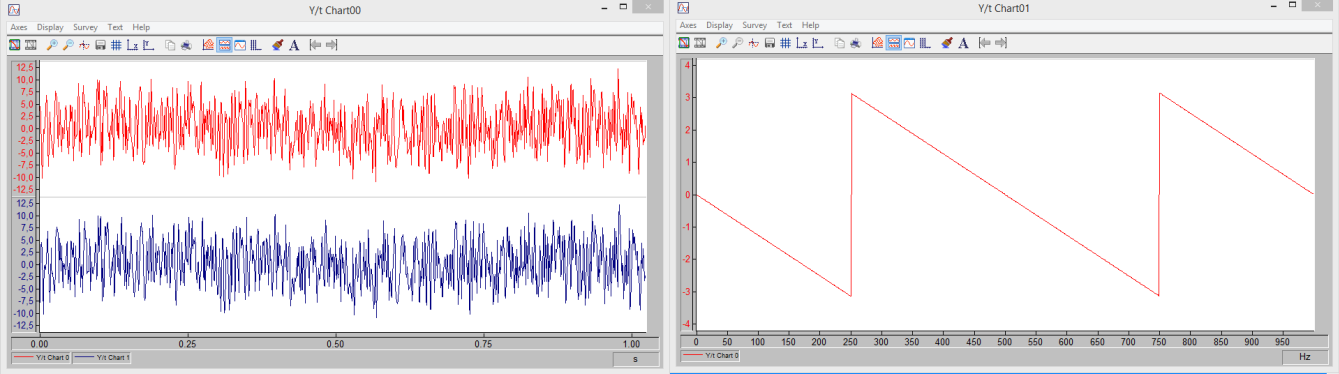
\includegraphics[width=1\linewidth]{wyk5}
\caption{Charakterystyka fazowa WGWM, dla częstotliwości 10Hz. Opóźnienie równe $1,9972ms$, faza równa $-2,57rad$, liczba uśrednień 40}
\label{fig:wyk5}
\end{figure}

\begin{figure}[H]
	\centering
	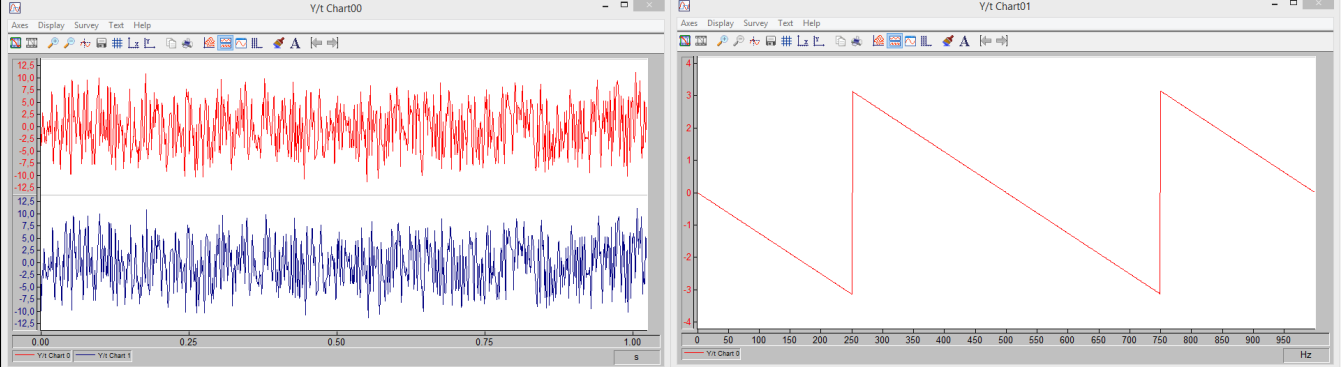
\includegraphics[width=1\linewidth]{wyk6}
	\caption{Charakterystyka fazowa WGWM, dla częstotliwości 100Hz. Opóźnienie równe $2,0023ms$, faza równa $-1,27rad$, liczba uśrednień 40 }
	\label{fig:wyk6}
\end{figure}


Przedstawione przebiegi na rys. \ref{fig:wyk5}, \ref{fig:wyk6}  wartości opóźnienia i fazy pokazały, że im wyższa częstotliwość nastawiona na module Slider00, tym bliższy jest wynik oczekiwany.

\subsection{Układ z schematu 2 rozbudować o dodatkowe moduły umożliwiające symulacje zakłóceń w sygnale opóźnionym (rys. \ref{fig:sch3})}

\begin{figure}[H]
\centering
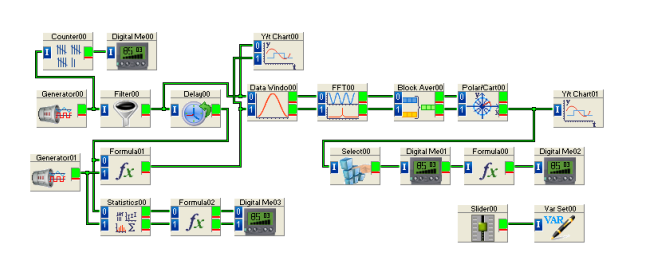
\includegraphics[width=0.7\linewidth]{sch3}
\caption{Układ z symulacja zakłóceń sygnału opóźnionego}
\label{fig:sch3}
\end{figure}

Sprawdzono działanie układu i poprawność pomiaru opóźnienia dla wybranej wartości częstotliwości (np. 200 Hz) i kilku wartości stosunku sygnał/szum. Zmieniając amplitudę szumu w module Generator01  w zakresie 1÷10 V.

\begin{figure}[H]
\centering
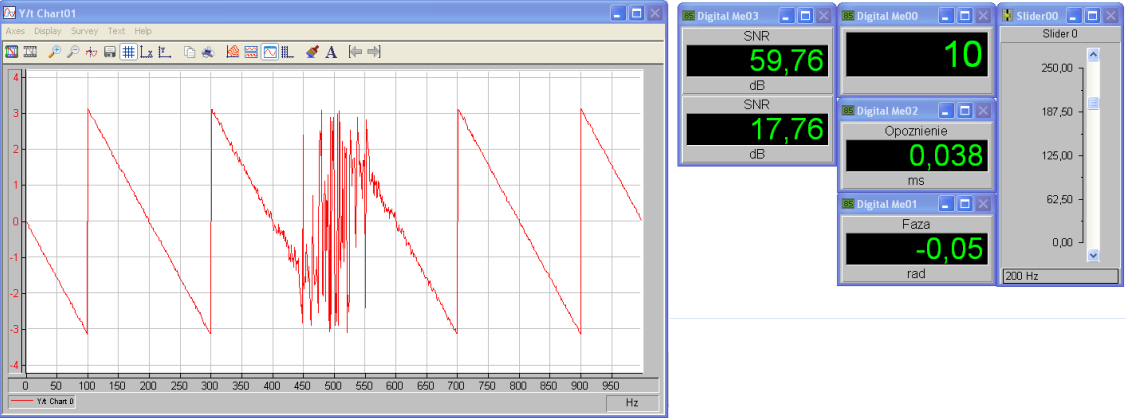
\includegraphics[width=0.8\linewidth]{wyk7}
\caption{Wyznaczone charakterystyki fazowe oraz wartości liczbowe: liczby uśrednień, wyznaczonego opóźnienia, wartości fazy oraz SNR dla $f_0 =200 Hz$ oraz amplitudzie sygnału szumu$U_m=7V$.}
\label{fig:wyk7}
\end{figure}

\begin{figure}[H]
	\centering
	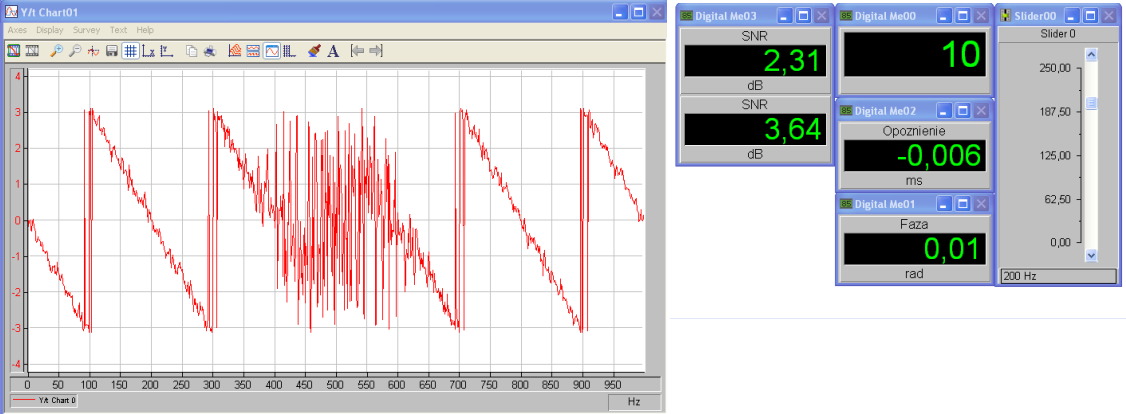
\includegraphics[width=0.8\linewidth]{wyk8}
	\caption{Wyznaczone charakterystyki fazowe oraz wartości liczbowe: liczby uśrednień, wyznaczonego opóźnienia, wartości fazy oraz SNR dla $f_0 =200 Hz$ oraz amplitudzie sygnału szumu $U_m=6V$}
	\label{fig:wyk8}
\end{figure}

\begin{figure}[H]
	\centering
	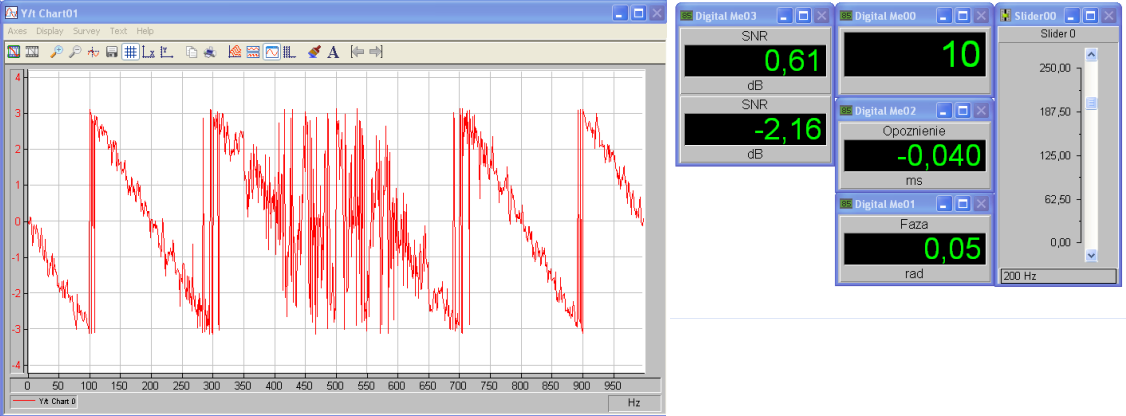
\includegraphics[width=0.8\linewidth]{wyk9}
	\caption{Wyznaczone charakterystyki fazowe oraz wartości liczbowe: liczby uśrednień, wyznaczonego opóźnienia, wartości fazy oraz SNR dla $f_0 =200 Hz$ oraz amplitudzie sygnału szumu $U_m= 9V$.}
	\label{fig:wyk9}
\end{figure}
Zaobserwowaliśmy że im wyższa amplituda zakłócenia od sygnał opóźnionego tym potrzebna wyższej liczby uśrednień jaką należy przeprowadzić w celu wyznaczenia wartości owego opóźnienia. Dla przypadku z rysunku \ref{fig:wyk9} , gdzie amplituda $U_m=9V$ potrzebne było zrealizowanie większej liczby uśrednień , zaś otrzymany wynik i tak obarczony został błędem, podczas gdy dla $U_m =2V$ wynik był po chwili zbieżny.
\subsection{Do układu z schematy 3 dodać tor do wyznaczania funkcji koherencji (rys. \ref{fig:sch4} ).}

\begin{figure}[H]
\centering
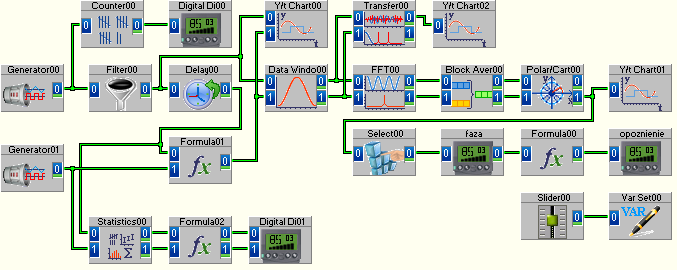
\includegraphics[width=0.7\linewidth]{sch4}
\caption{Tor do wyznaczania funkcji koherencji.}
\label{fig:sch4}
\end{figure}

Zmieniając amplitudę szumu w module Generator01 w zakresie 1÷10 V zaobserwowano przebieg funkcji koherencji.

\begin{figure}[H]
	\centering
	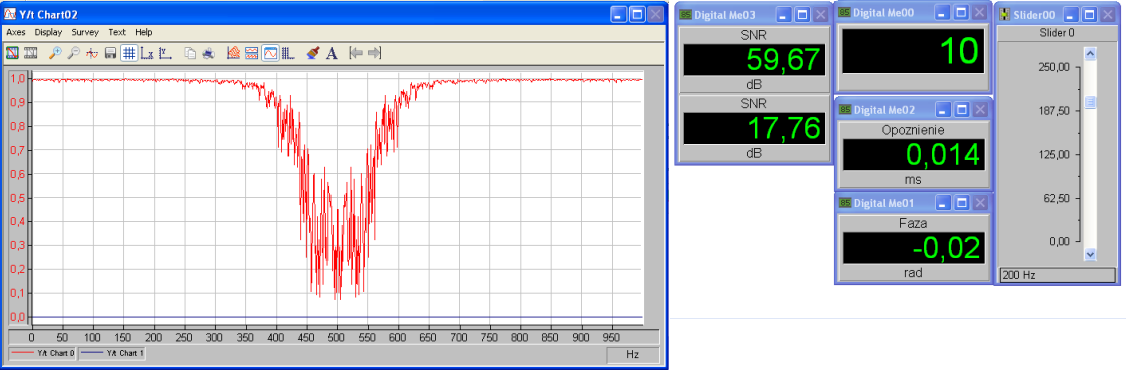
\includegraphics[width=0.8\linewidth]{wyk12}
	\caption{Funkcja koherencji dla amplitudy zakłócenia Um=1V}
	\label{fig:wyk12}
\end{figure}

\begin{figure}[H]
\centering
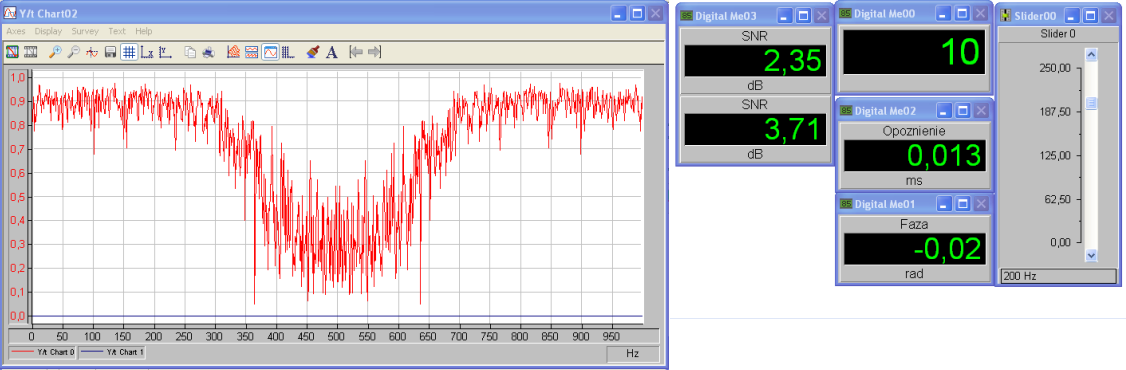
\includegraphics[width=0.8\linewidth]{wyk11}
\caption{Funkcja koherencji dla amplitudy zakłócenia Um=6V }
\label{fig:wyk11}
\end{figure}

Koherencja jest funkcją częstotliwości pokazującą jaki jest współczynnik korelacji pomiędzy dwoma procesami stochastycznymi zależny od częstotliwości. Wysoka koherencja dla danej częstotliwości wskazuje na to, że dwa sygnały mają wysoką koncentrację mocy dla tej częstotliwości. Następną własnością koherencji jest możliwość pomiaru wzajemnego kąta fazowego pomiędzy dwoma sygnałami w funkcji częstotliwości. Sygnały mogą mieć różnice faz równą zero i wówczas są one synchroniczne lub różnice 180 stopni i wówczas są asynchroniczne

\subsection{Rozbudowano układ o tor do wyznaczania odchylenia standardowego opóźnienia (rys. \ref{fig:sch5})}

\begin{figure}[H]
\centering
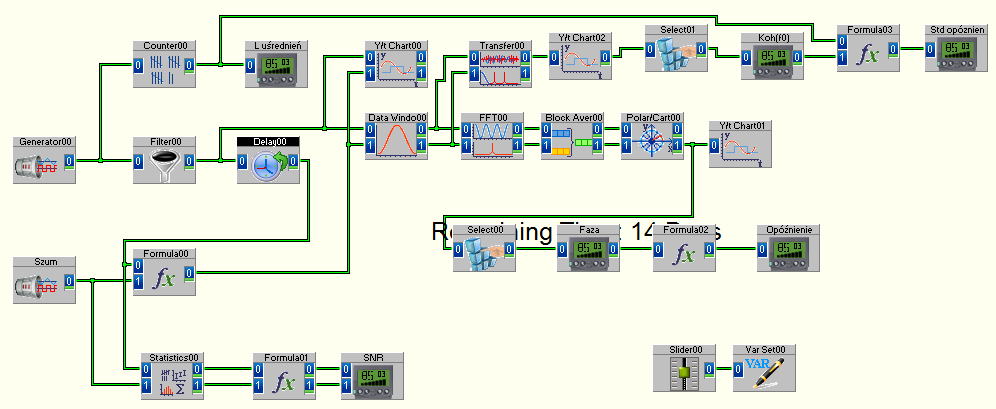
\includegraphics[width=0.8\linewidth]{sch5}
\caption{Układ do badania metody wyznaczania opóźnienia z fazy WGWM}
\label{fig:sch5}
\end{figure}

\begin{figure}[H]
\centering
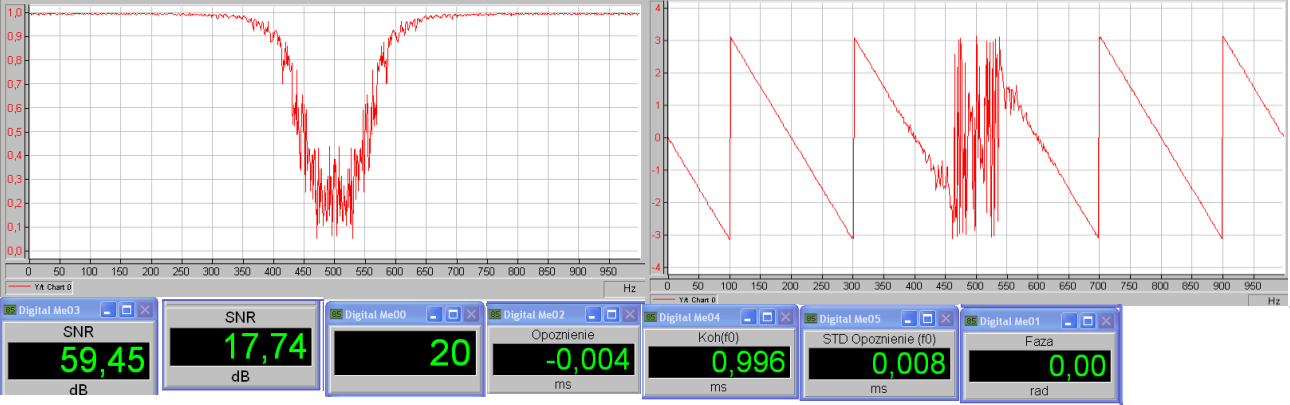
\includegraphics[width=0.8\linewidth]{wyk13}
\caption{ Wyznaczone charakterystyki fazowe (1)}
\label{fig:wyk13}
\end{figure}


\begin{figure}[H]
	\centering
	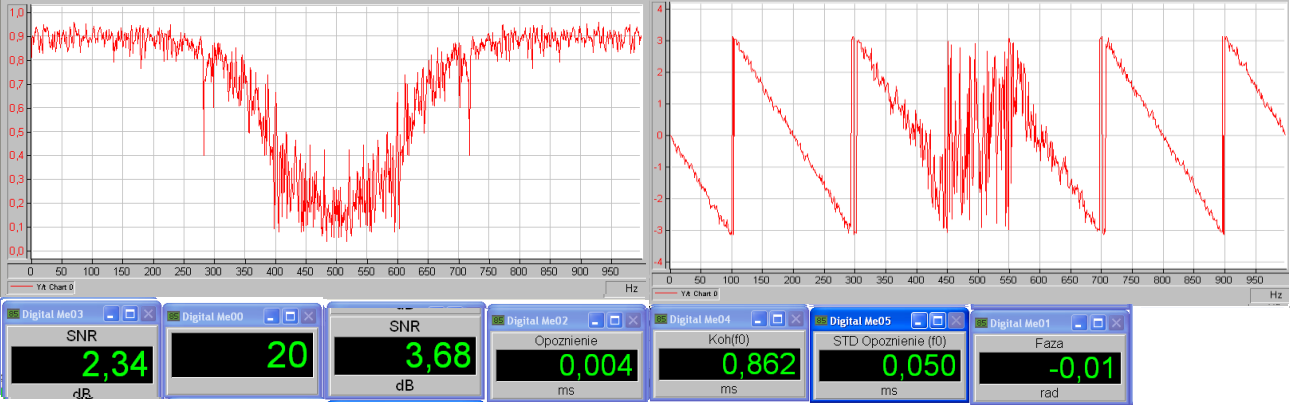
\includegraphics[width=0.8\linewidth]{wyk14}
	\caption{ Wyznaczone charakterystyki fazowe (2)}
	\label{fig:wyk14}
\end{figure}

\begin{figure}[H]
	\centering
	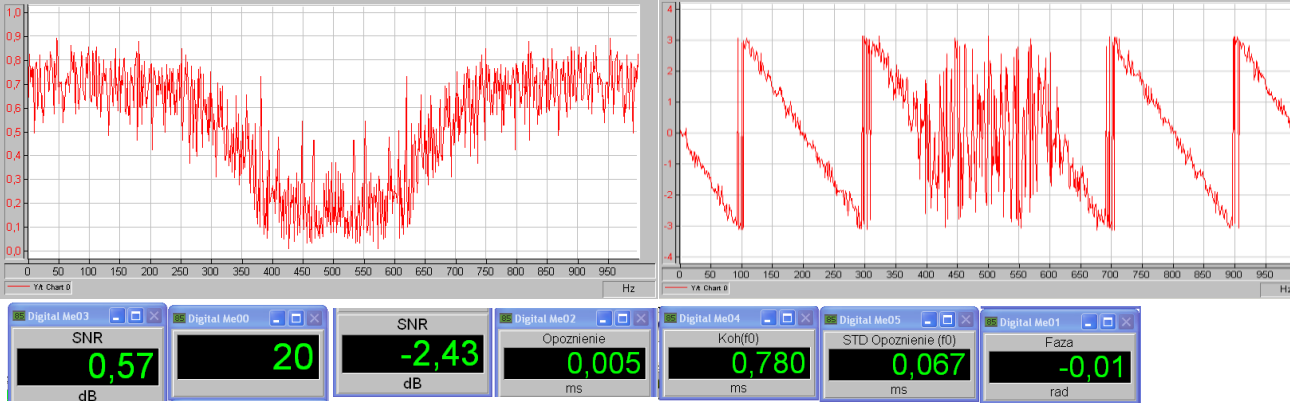
\includegraphics[width=0.8\linewidth]{wyk15}
	\caption{ Wyznaczone charakterystyki fazowe (3)}
	\label{fig:wyk15}
\end{figure}

\begin{figure}[H]
	\centering
	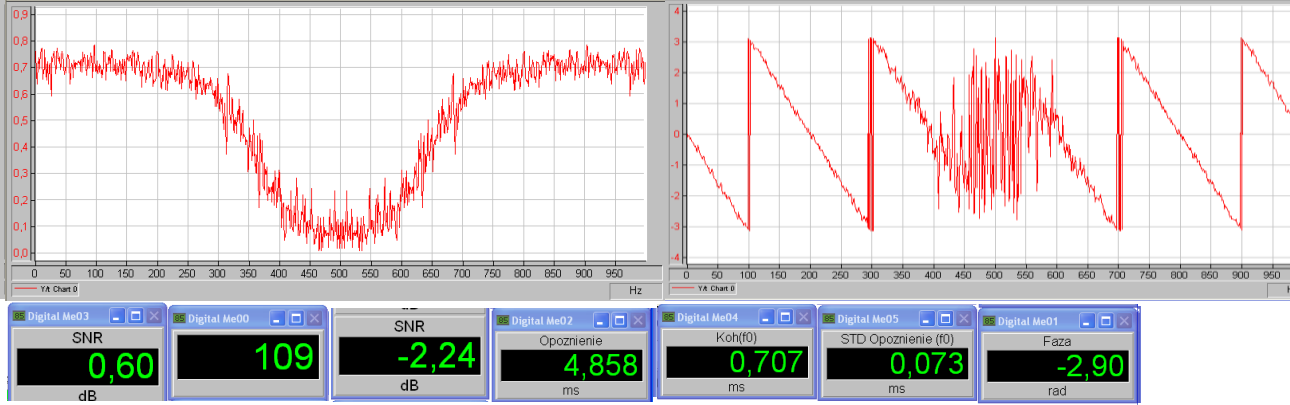
\includegraphics[width=0.8\linewidth]{wyk16}
	\caption{ Wyznaczone charakterystyki fazowe (4)}
	\label{fig:wyk16}
\end{figure}

Poniżej zostały zestawione powyższe dane z wykresów

\begin{table}[H]
	\centering
	\caption{Tabela pomiarowa}
	\label{my-label}
	\begin{tabular}{|l|l|l|l|l|}
		\hline
		lp.             & 1      & 2     & 3     & 4     \\ \hline
		$f_0$           & 200    & 200   & 200   & 200   \\ \hline
		SNR             & 59,45  & 2,34  & 0,57  & 0,59  \\ \hline
		SNR             & 17,74  & 3,68  & -2,43 & -2,29 \\ \hline
		usr.            & 20     & 20    & 20    & 300   \\ \hline
		opuznienie      & -0,004 & 0,004 & 0,005 & 0,013 \\ \hline
		Opuzninie $f_0$ & 0,008  & 0,05  & 0,067 & 0,021 \\ \hline
		faza            & 0      & -0,01 & -0,01 & -0,02 \\ \hline
		$K_{oh(f_{0})}$ & 0,996  & 0,862 & 0,78  & 0,71  \\ \hline
	\end{tabular}
\end{table}

Przy doborze wartości SNR trzeba zwrócić uwagę na opóźnienia, liczbę uśrednień oraz częstotliwość $f_0$. Najlepszą wartość SNR można uzyskać przy jak najmniejszych szumach jednak jest to przypadek idealny i nie występuje w rzeczywistości.


\begin{thebibliography}{0}
  \bibitem{l2short} Robert Hanus, \textsl{Instrukcje laboratoryjne,} Politechnika Rzeszowska, Rzeszów, 2015
\end{thebibliography}
\end{document}
